\documentclass[11pt,letterpaper,twocolumn]{article} % {{{
\usepackage[utf8]{inputenc}
\usepackage[spanish]{babel}
\usepackage{amsmath}
\usepackage{amsfonts}
\usepackage{amssymb}
\usepackage{graphicx}
\graphicspath{{img/}}
\usepackage{physics}
%\usepackage{bbm}|
\usepackage[dvipsnames]{xcolor}
\usepackage[margin=1in]{geometry}
\usepackage{booktabs}
\usepackage{float}

\newcommand{\eref}[1]{eq.~(\ref{#1})} 
\newcommand{\sref}[1]{sec.~\ref{#1}}
\newcommand{\fref}[1]{Fig.~\ref{#1}}
\newcommand{\tref}[1]{table~\ref{#1}}
\newcommand{\Eref}[1]{Eq.~(\ref{#1})} 
\newcommand{\Sref}[1]{Sec.~\ref{#1}}
\newcommand{\Fref}[1]{Fig.~\ref{#1}}  
\newcommand{\Tref}[1]{Table~\ref{#1}}

\usepackage{hyperref}
\hypersetup{
colorlinks=true,
linkcolor=blue,
filecolor=blue,      
citecolor=blue,
urlcolor=blue,
pdftitle={},
pdfauthor=author={Jose Alfredo de Leon},
}

\usepackage{tikz}

%\usepackage[mathlines]{lineno}  \linenumbers \setlength\linenumbersep{5pt}
%\usepackage[inline]{showlabels,rotating}
%\renewcommand{\showlabelrefline}{\hrule width 0pt height 3ex depth 0pt}
%\renewcommand{\showlabelfont}{\small\slshape\color{red!70}}
\usepackage[draft,inline,nomargin]{fixme} \fxsetup{theme=color}
\definecolor{jacolor}{RGB}{200,40,0} \FXRegisterAuthor{ja}{aja}{\color{jacolor}JA}
\FXRegisterAuthor{cp}{acp}{\color{blue}CP}
\FXRegisterAuthor{cd}{acd}{\color{purple}CD}

\decimalpoint

\newcommand{\mbZ}{\mathbb{Z}}
\newcommand{\mcH}{\mathcal{H}}
\newcommand{\mcD}{\mathcal{D}}
\newcommand{\mcDPT}{\mathcal{D}^{T_B}}
\newcommand{\mcG}{\mathcal{G}}
\renewcommand{\H}{\h\in g}
\def\bbra#1{\mathinner{\langle \! \langle{#1}|}}
\def\kket#1{\mathinner{|{#1}\rangle \! \rangle}}
\def\ddyada#1{\mathinner{|{#1}\rangle\!\rangle\!\langle\!\langle{#1}|}}
\def\ddyad#1#2{\mathinner{|{#1}\rangle\!\rangle\!\langle\!\langle{#2}|}}
\def\bbrakket#1#2{\mathinner{\langle\!\langle {#1}|{#2}\rangle\!\rangle}}
\def\brakket#1#2{\mathinner{\langle {#1}|{#2}\rangle\!\rangle}}
\def\bbraket#1#2{\mathinner{\langle\!\langle {#1}|{#2}\rangle}}
\newcommand{\h}{\qty(m, n)}
\newcommand{\vh}{\qty(\vec m,\vec n)}

\newcommand{\one}{\mathbbm{1}}
\newcommand{\mcF}{\mathcal{F}}

\newtheorem{theorem}{Teorema}
\newtheorem{proof}{Demostración}
\newtheorem{hypothesis}{Hipótesis}

\title{The simplest discrete-time quantum walk producing Parrondo's paradox}
\author{}
\date{Última actualización: \today}

\renewcommand{\labelenumii}{\arabic{enumi}.\arabic{enumii}}
\renewcommand{\labelenumiii}{\arabic{enumi}.\arabic{enumii}.\arabic{enumiii}}
\renewcommand{\labelenumiv}{\arabic{enumi}.\arabic{enumii}.\arabic{enumiii}.\arabic{enumiv}}

\newcommand{\rhoel}[2]{\rho_{#1,#2} \dyad{#1}{#2}}
\newcommand{\p}{p_{\text{error}}}

\begin{document}
\maketitle

%\section*{Introduction}
%
%Parrondo's paradox, a counterintuitive phenomenon first observed in
%classical gambling games, demonstrates that two individually losingd
%strategies can, when combined in a specific sequence, lead to a winning    
%outcome \cite{Parrondo1996, Harmer1999}. This captivating effect
%challenges classical intuition and has found applications and
%theoretical interest across diverse fields, ranging from economics and
%biology to engineering and social sciences \cite{Davis1999, Abbott2001,
%Arena2018}. Its ubiquity underscores the complex interplay between
%seemingly disadvantageous components that, through non-linear
%combination, yield an emergent advantageous macroscopic behavior.
%
%The advent of quantum mechanics has opened new avenues for exploring such
%paradoxical behaviors, particularly within the framework of quantum
%walks \cite{Aharonov1993, Ambainis2001}. Quantum walks, the quantum
%analogues of classical random walks, are fundamental processes in
%quantum information science, providing a powerful model for quantum
%computation, algorithm design, and quantum simulation \cite{Venegas2012,
%Kempe2003, Childs2009}. Unlike their classical counterparts, quantum
%walks exhibit unique features such as superposition and quantum
%interference, which lead to distinct spreading patterns and dynamics
%\cite{Konno2005, Mielke2015}. These inherent quantum properties suggest a
%richer landscape for the manifestation and manipulation of phenomena
%like Parrondo's paradox, potentially offering insights into the
%boundaries of classical and quantum behavior \cite{Meyer1996, Flitney2007}.
%
%Initial investigations into the realization of Parrondo's paradox within
%discrete-time quantum walks (DTQWs) primarily focused on single-particle
%walks on a one-dimensional line \cite{Chandrashekar2011}. Early studies,
%employing simple, fixed coin operators, encountered challenges in
%robustly demonstrating the genuine Parrondo's effect, particularly its
%persistence over a large number of steps or in scenarios involving only
%two static, homogeneous ``losing'' games \cite{Pakkonen2014,
%Rajendran2018}. It was often posited that complex time-dependent or
%spatially inhomogeneous coin operations, or specific measurement
%strategies, were necessary to observe the paradox effectively, suggesting
%that the simplicity of the classical paradox might not directly translate
%to the quantum realm under straightforward conditions \cite{Mittal2024,
%Walczak2025, Pires2020}. This perception created a theoretical gap,
%prompting further exploration into the minimal conditions required for
%its emergence.
%
%In this paper, we address this fundamental question by presenting a
%comprehensive investigation into the simplest form of Parrondo's paradox
%in discrete-time quantum walks, utilizing only two distinct, homogeneous
%coin operators. Specifically, we model these operations as fixed
%rotations of the Bloch sphere, representing the two ``losing'' quantum
%games \cite{Nielsen2000, Phoenix2002}. Our objective is to rigorously
%establish the conditions under which these two individually detrimental
%quantum operations, when combined in alternating sequences, yield a net
%``winning'' outcome for the quantum walker, defined by the expectation
%value of its position \cite{Rajendran2018, Chandrashekar2011}. By
%focusing on such a minimalist setup, we aim to uncover the essential
%quantum mechanical principles, particularly the role of interference,
%that facilitate the paradox's emergence and persistence without recourse
%to complex time- or position-dependent parameters.
%
%Our findings demonstrate that, contrary to some earlier assumptions, a
%genuine Parrondo's paradox can indeed be robustly observed in DTQWs with
%appropriately chosen, yet homogeneous, two-state coin operators \cite{Mihai2018,
%Mancino2022}. We analytically derive and numerically confirm the
%parameter regimes for these Bloch sphere rotations and the initial coin
%state that allow for the paradox's manifestation. This work not only
%provides a foundational understanding of Parrondo's paradox in its
%simplest quantum embodiment but also sheds light on the subtle interplay
%between quantum coin biases, interference effects, and the combinatorial
%strategy \cite{Kadiri2024}. The implications extend to quantum game
%theory, quantum simulation, and potentially inspire new approaches for
%designing quantum algorithms where counterintuitive collective behavior
%can be harnessed for advantageous outcomes.
%
%\break

% Read the following introduction and re-write the first sentence of the second
% parragraph ("quantum mechanics provides a fascinating...") to make it less
% pompous and more sober, more serious and more adequate for a research
% paper to be submitted at Physical review. Return only the re-writen 
% sentence
\section{Introduction}

Parrondo's Paradox, a counterintuitive phenomenon first observed in classical
game theory, demonstrates that two individually losing strategies can combine
in a specific sequence to yield an overall winning outcome. This intriguing
effect, initially conceptualized as a pedagogical model for the Brownian
ratchet, arises from the nonlinear interaction between the strategies. Its
implications extend beyond games, offering insights into systems ranging from
economics to biology.

Quantum mechanics offers a natural setting to revisit classical paradoxes, often 
revealing new behavior stemming from principles such as superposition and 
interference. Quantum walks, the quantum analogs of classical random walks, 
have gained more and more attention for this exploration. 
Unlike their classical counterparts, quantum walks exhibit
ballistic spreading rather than diffusive, driven by quantum coherence.
This fundamental difference suggests that Parrondo's Paradox, when translated
to quantum walk systems, could manifest under distinct and perhaps simpler
conditions than in its classical setting. A typical discrete-time quantum
walk (DTQW) involves a quantum particle (the walker) on a lattice, equipped with an
internal degree of freedom known as the coin state. At each step, a
unitary operator acts on this internal state emulating \textit{tossing a quantum coin}, creating a
superposition, followed by a conditional shift operator that moves the
walker based on its coin state.

Previous research has explored various avenues for realizing Parrondo's Paradox
in quantum walks. Early theoretical studies demonstrated the paradox using
alternating or combining different quantum coin operators, leveraging
interference effects from phase factors to reverse bias \cite{chandrashekar2011,flitney2012, li2013}. The paradox has been shown to emerge from
history-dependent coin operations \cite{flitney2004} and has even been
observed with higher-dimensional quantum coins, such as three-state
(qutrit) or four-sided coins, sometimes requiring a classical ratcheting effect
\cite{rajendran2018playing, lai2020parrondo, walczak2022parrondo}. More recently,
explorations have expanded to include time-dependent and spatially
inhomogeneous coin operators \cite{pires2020parrondo, mittal2024parrondo,
walczak2025parrondo}, different shift operators \cite{walczak2024parrondo},
and even the unexpected role of noise \cite{walczak2023noise} or
spontaneous emission \cite{bolik2024spontaneous} in inducing or enhancing
the paradox. The effect has also been theoretically extended to
continuous-time quantum walks with defect modulation \cite{ximenes2024parrondo}
and explored in the context of quantum search algorithms
\cite{hosaka2024parrondo}. Furthermore, the interplay between Parrondo's Paradox
and quantum entanglement has been a significant focus, with studies
showing how Parrondo sequences can generate highly entangled states
\cite{panda2022generating, jan2023territories} and, conversely, how entanglement
dynamics are affected by the paradox \cite{walczak2021parrondo,
walczak2023noise, walczak2025parrondo}. Experimental realization of the paradox
in 1D quantum walks has also been successfully achieved using optical setups
\cite{jan2020experimental}, validating theoretical predictions.

Despite these diverse demonstrations, a systematic and simplified approach to
inducing Parrondo's Paradox in discrete-time quantum walks using only the
combination of two homogeneous coin rotations from SU(2), without
recourse to position-dependent coins, complex higher-dimensional coins, or
external noise, has remained elusive. Such a minimal setup would provide clearer
insight into the fundamental quantum mechanisms underlying the paradox.

In this paper, we present the first systematic demonstration of Parrondo's
Paradox in the simplest discrete-time quantum walk model. We show how to
combine two individually losing games, each defined by a distinct homogeneous
coin operation that is a rotation within SU(2), to produce an overall winning
outcome. Our methodology meticulously outlines the conditions under which these
two simple, unbiased coin operations, when applied in a specific sequence, lead
to a rectified average position of the quantum walker. These results represent a
significant simplification of prior realizations and offer a foundational
understanding of the paradox's emergence from the interplay of quantum
interference and unitary transformations alone.

\begin{figure}
\centering
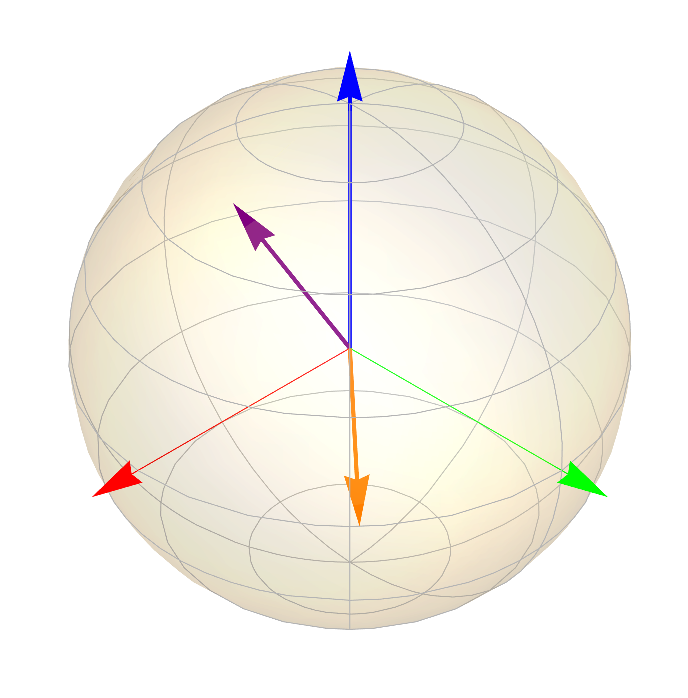
\includegraphics[width=0.37\textwidth]{figs/fixed_rotation_axes_bloch_sphere_01.pdf}
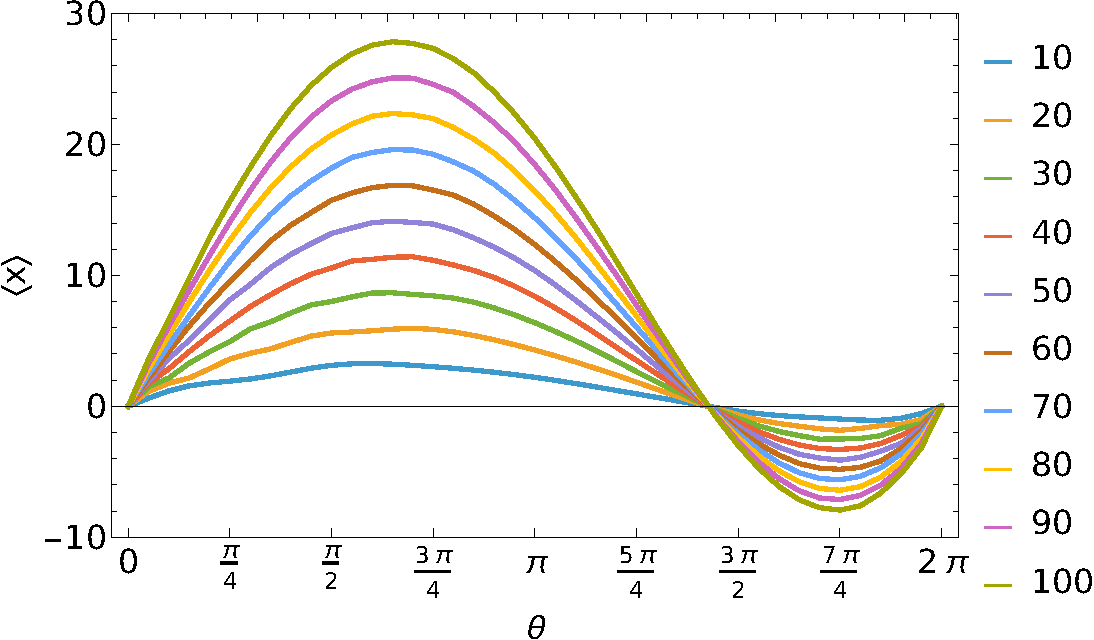
\includegraphics[width=0.6\textwidth]{figs/fixed_rotation_axes_expval_01.pdf}
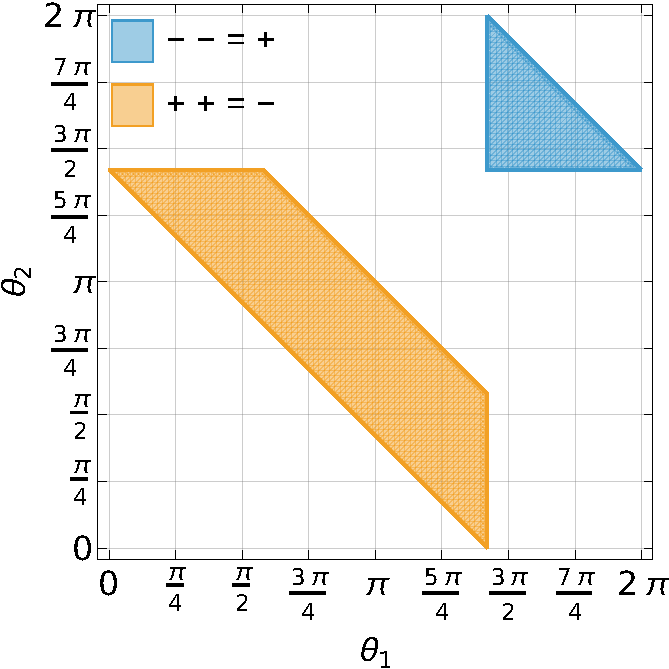
\includegraphics[width=0.7\textwidth]{figs/fixed_rotation_axes_01.pdf}
\caption{$\ket{\psi_0(\theta,\phi)} = \ket{\psi_0(0.5\pi, 0.26\pi)}$, 
eje de rotación: $(\alpha, \phi) = (0.18\pi, 0)$}
\end{figure}

%	Verificar si tomos dos ejes arbitrarios tampoco depende de phi, convencerme
%	Escribir lo de t parrondo
% 

\bibliographystyle{unsrt}
\bibliography{references.bib,references2.bib}
\end{document}